


\newcommand{\FigHighLevel}{
\begin{figure}[ht]
    \centering
    % 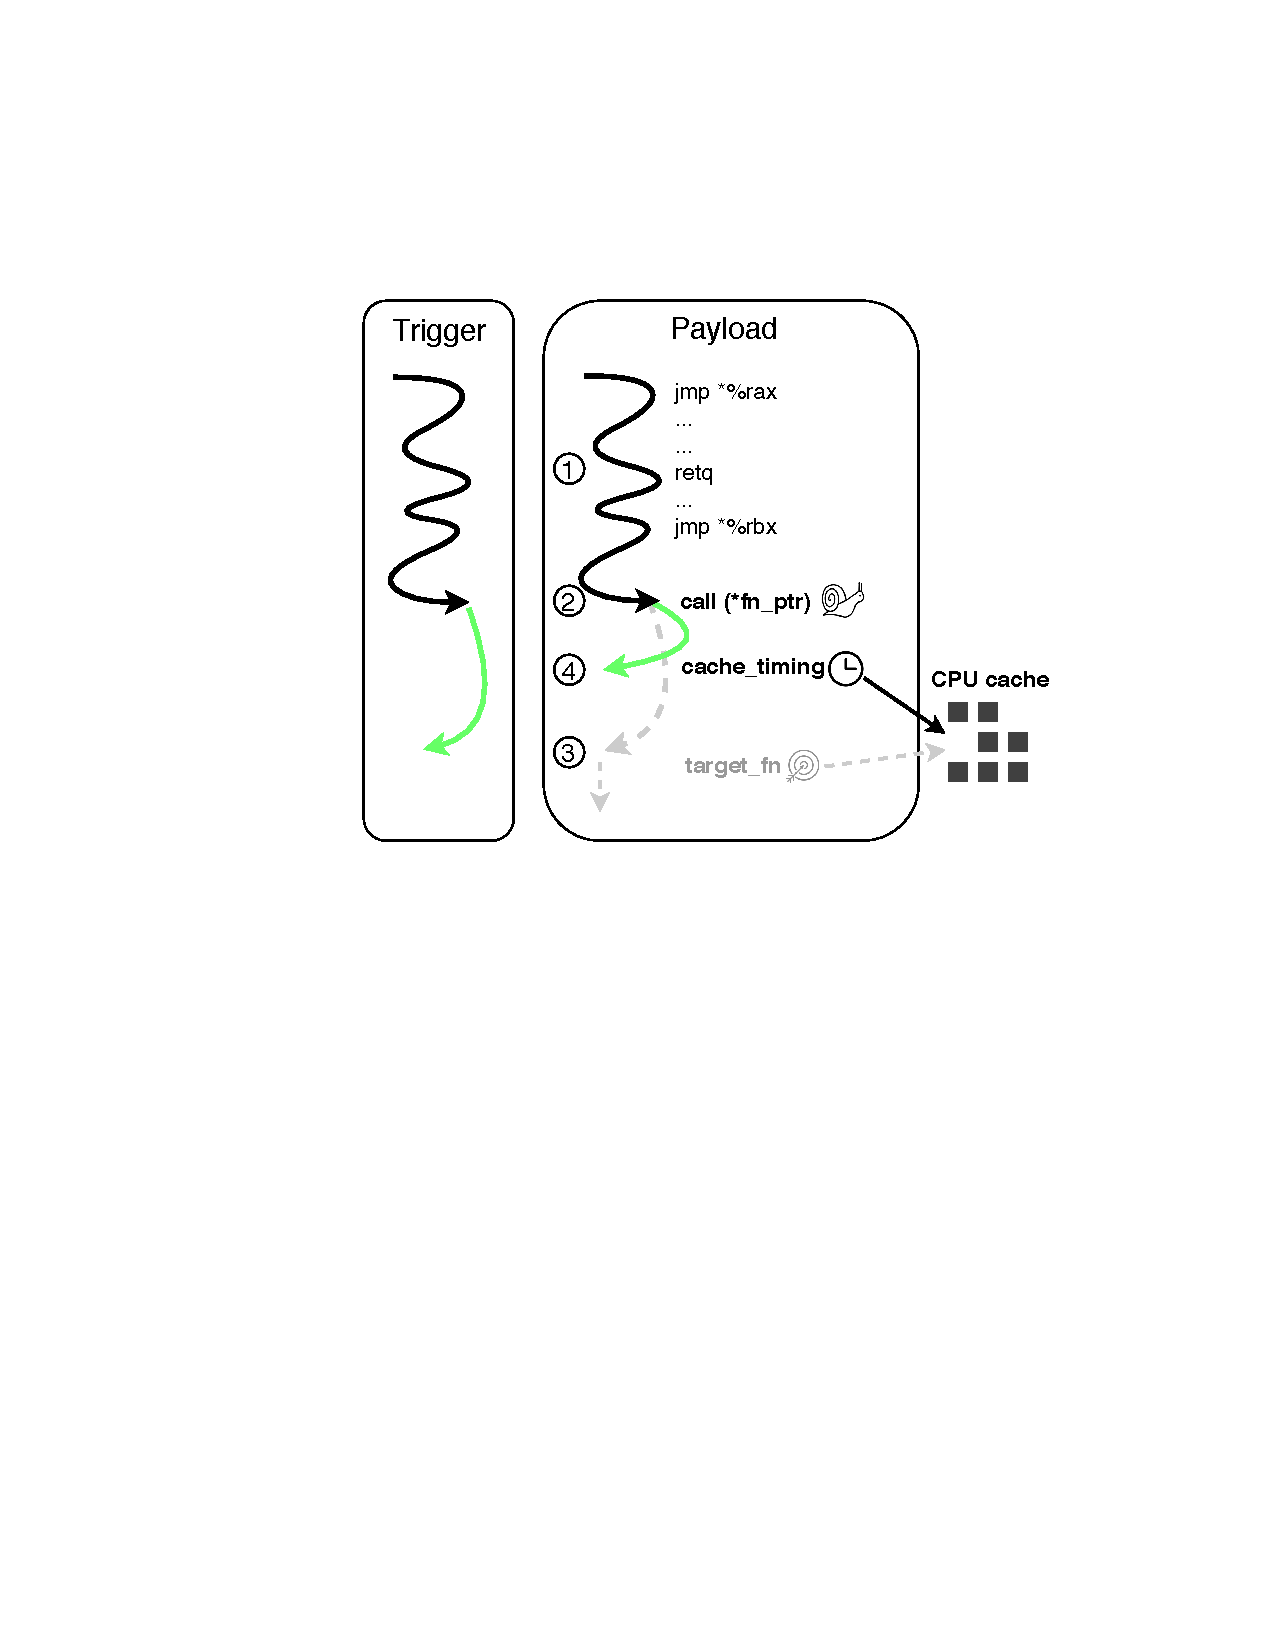
\includegraphics[clip, trim=6cm 13.5cm 3.8cm 5cm, width=0.9\linewidth]{figures/exspectre-high-level.pdf}
    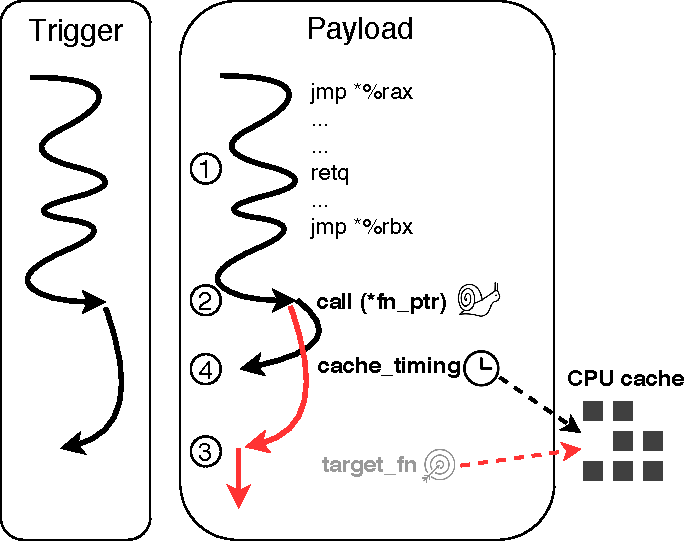
\includegraphics[width=0.9\linewidth]{figures/exspectre-high-level-new.pdf}
    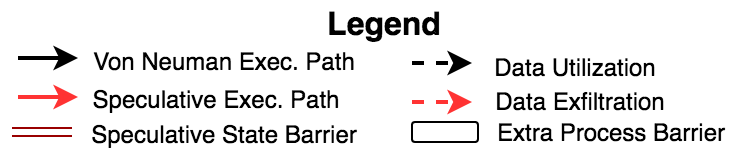
\includegraphics[width=0.4\textwidth]{figures/ExSpectre_CR_key.png}
    \caption{\textbf{\speculake}\,---\,%
    Both the trigger and payload binaries exhibit the same initial series of
    indirect jumps (Step 1). The trigger program solely executes these
    jumps to (mis)train the branch predictor. In the Payload program
    \texttt{fn\_ptr} has been set to point to the \texttt{cache\_timing}
    function and flushed from cache. Thus the branch predictor
    mis-predicts the jump to \texttt{cache\_timing} and instead jumps to
    \texttt{target\_fn} (Step 2) as trained by the trigger program (green line). 
    \texttt{target\_fn} then executes speculatively (Step 3), until
    \texttt{fn\_ptr} is loaded from memory and the processor redirects
    computation to the \texttt{cache\_timing} function (Step 4),
    which measures which value was speculatively loaded into cache.}
    \label{fig:high-level}

\end{figure}
}


\newcommand{\FigNestedSpec}{
\begin{figure}[t]
    \centering
    % 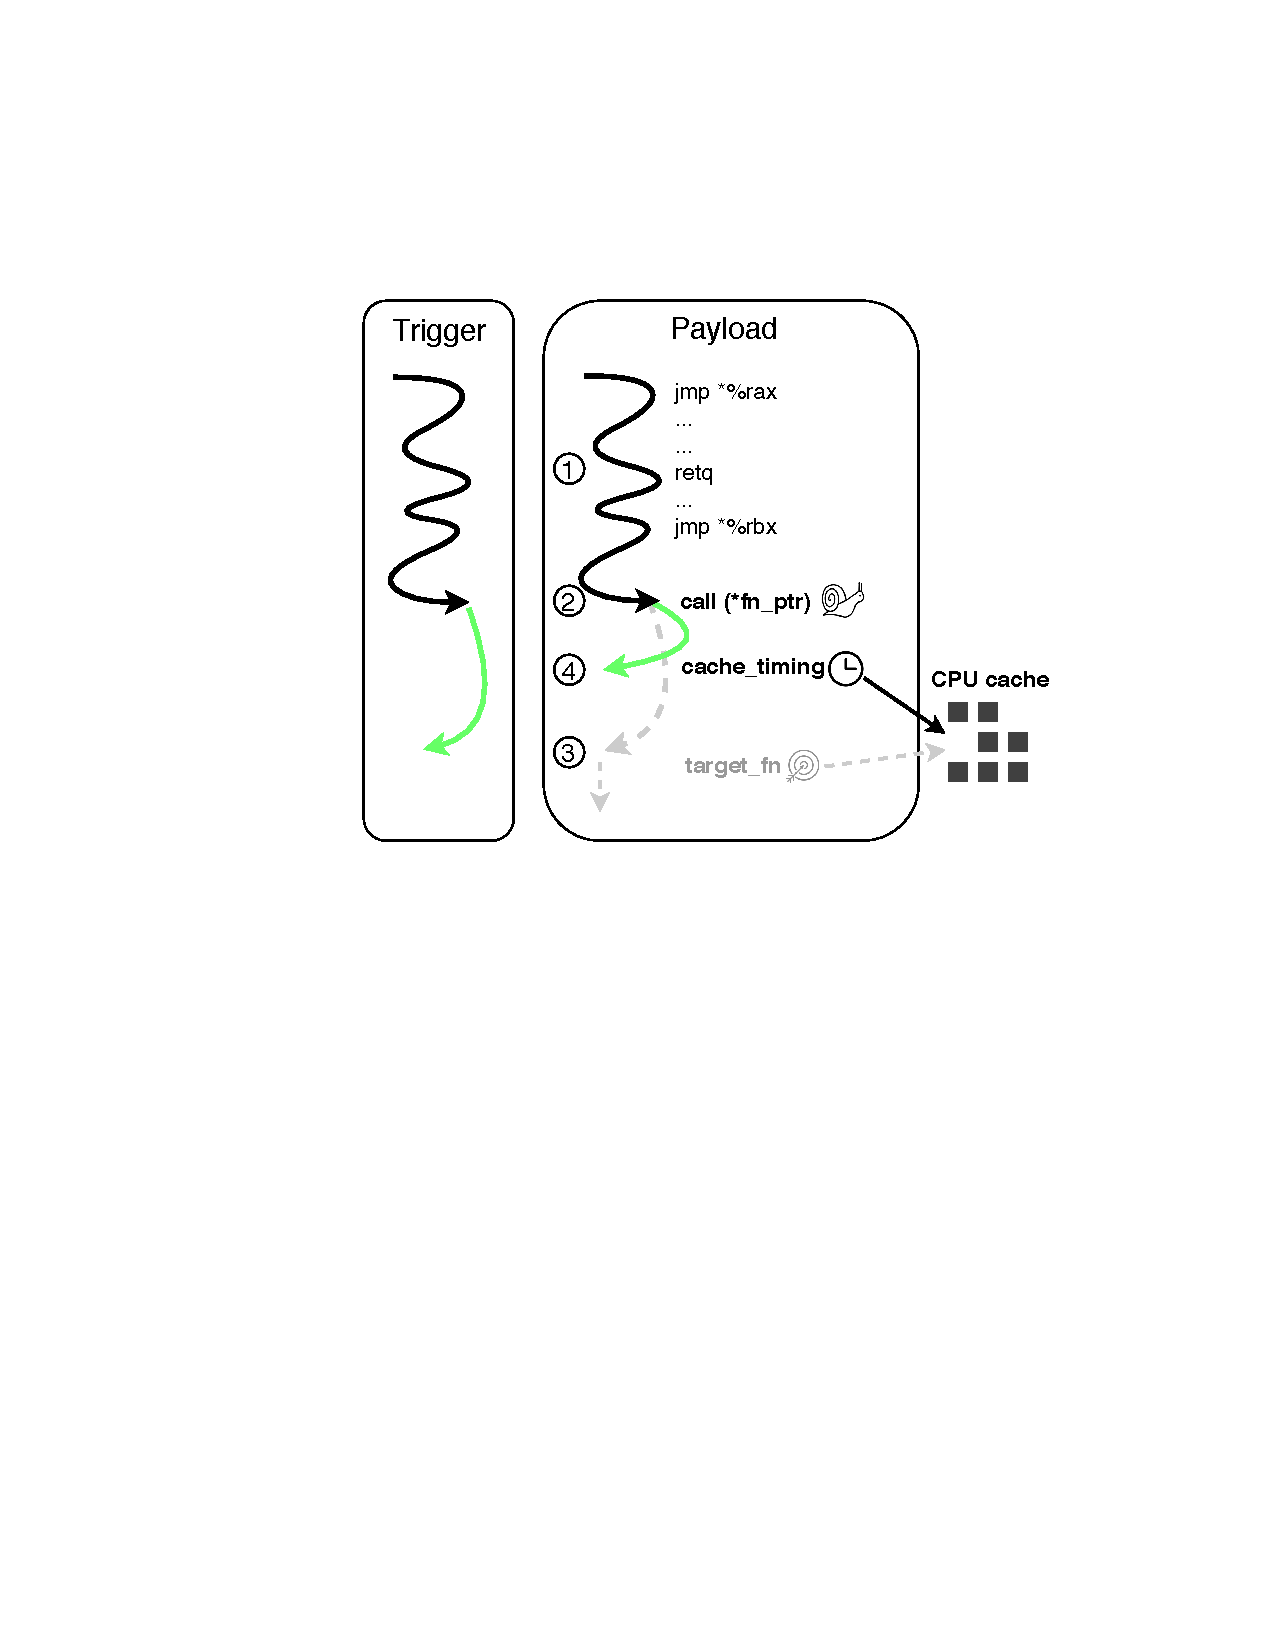
\includegraphics[clip, trim=6cm 13.5cm 3.8cm 5cm, width=0.9\linewidth]{figures/exspectre-high-level.pdf}
    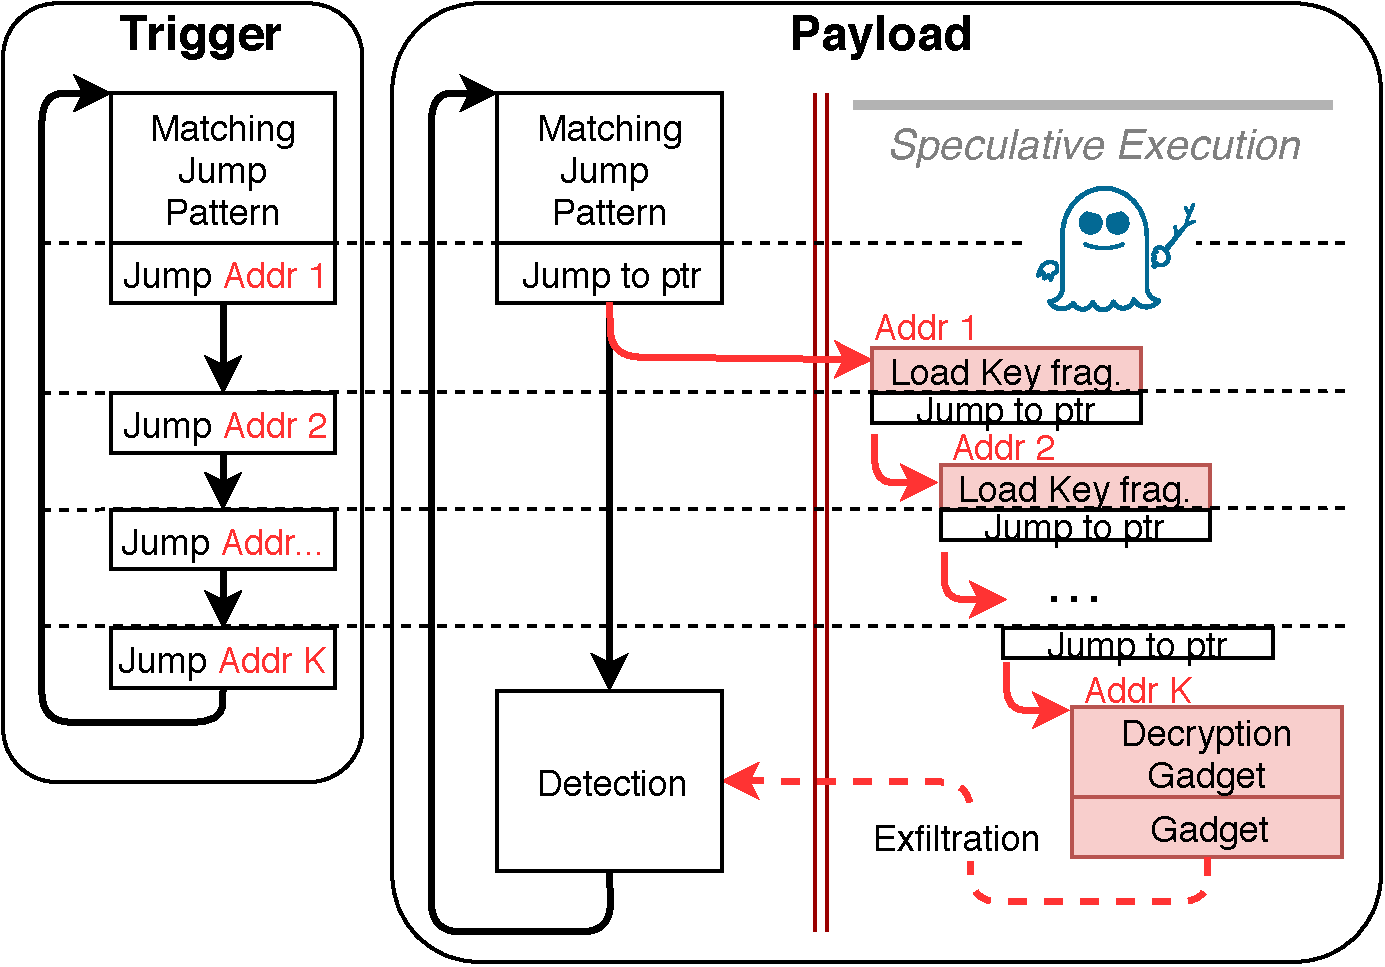
\includegraphics[width=0.95\linewidth]{figures/ExSpectre_CR_Nested.pdf}
    \caption{\textbf{Nested Speculation}\,---\,%
    Using nested speculation for obfuscated key derivation. The payload uses 
    a sequence of indirect jumps controlled by the trigger to incrementally 
    construct a key exclusively in the speculative environment. Without the 
    trigger an analyst will need to evaluate every ordering of \textbf{all} indirect 
    jumps to reconstruct the key. While the \textit{decryption gadget} may be trivial 
    for an analyst to find, this allows for an encrypted blob in the payload 
    to remain inaccessible in the absence of the trigger. }
    \label{fig:nested-spec}    

\end{figure}
}


\newcommand{\FigSpectreOne}{
\begin{figure}[t]
    \centering
    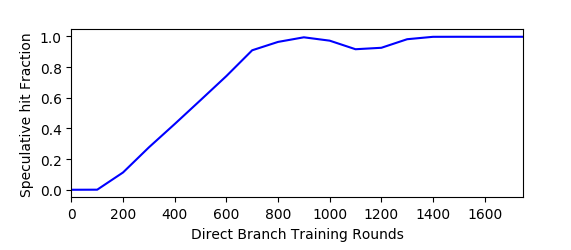
\includegraphics[width=0.9\linewidth]{figures/spectre_1_training.png}
    \caption{\textbf{Speculative buffer overflow warm-up}\,---\,%
    The direct branch predictor must
    be trained to expect that a branch will go a specific way before speculative
    buffer overflows can be used. We varied the number of times a branch was trained
    to be taken and observed the fraction of times we achieved a speculative buffer overflow
    execution immediately after (measured by observing if a speculatively-loaded value was present
    in cache avgeraged over 20,000 trials). We find that a branch must be trained in a
    direction hundreds of times before it can start to be used in a speculative buffer overflow.}
    \label{fig:spectre-one}
\end{figure}
}


\newcommand{\FigSpectreOneModel}{
\begin{figure}[ht]
    \centering
    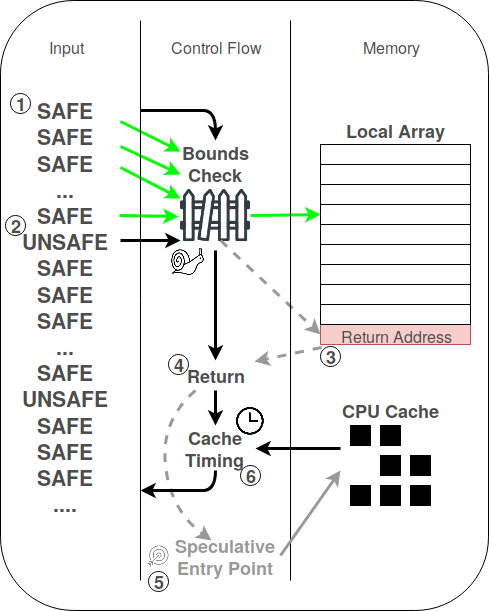
\includegraphics[width=0.9\linewidth]{figures/spectre_1_model.png}
    \caption{\textbf{Speculative Buffer Overflow}\,---\,%
    Safe input values are stored into a local array (Step 1),
    training the branch predictor to bypass the bounds check when given
    unsafe input (Step 2). This results in a speculative array store which
    overflows the bounds and overwrite a return address (Step 3). The CPU's 
    store-to-load forwarding will forward the speculative overflow to the 
    return (Step 4), where it will steer speculative execution to the 
    attacker-specified speculative entry point (Step 5). Eventually, the 
    original bounds check is resolved and control flow is redirected to the 
    cache timing function (Step 6). }
    \label{fig:spectre-one-model}
\end{figure}
}


\newcommand{\FigSpecMeasureNP}{
\begin{figure*}[t]
    \centering
    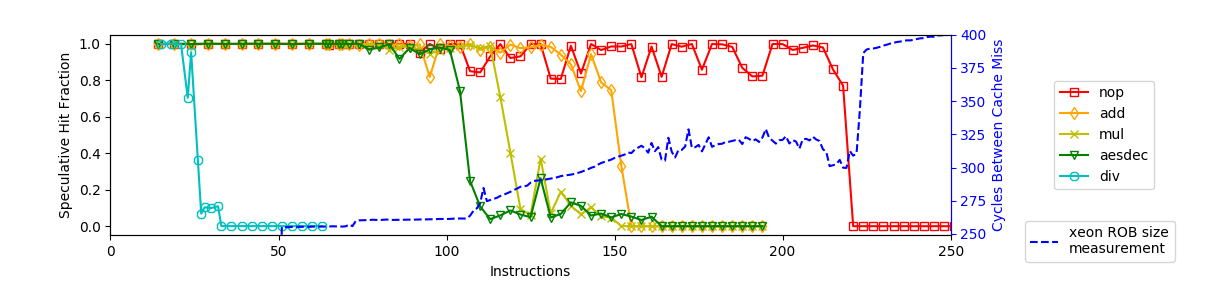
\includegraphics[width=0.9\textwidth]{figures/Speculative_measurements_no-parity.png}
    \caption{\textbf{Speculative limits}\,---\,%
    To find the number of instructions we can execute speculatively we placed a signal gadget
    after an increasing number of instructions and measured the fraction of times the 
    loaded value was subsequently in cache. However more complex instructions have stricter 
    constraints applied at two limits that we have identified, cache latency cycle limitation, and 
    the CPU's reorder buffer~(ROB) size as measured by instruction $\mu$-ops. We find that the
    hit fraction for instructions with a ratio of cycle latency to $\mu$~ops greater than 1 undergo a
    steep drop to \~0.1 hit fraction before falling definitively to 0. The drop in hit fraction 
    indicates that the duration of the test in cycles is beyond the fist step in cache latency as shown in 
    Figure~\ref{fig:cache-miss} (approx. 200 cycles). If the instruction sequence does not reach the 
    cycle count limit we see only a sharp drop in hit fraction to 0 indicating the limiting factor 
    is ROB size.  For example, the \texttt{idiv (r32)} instruction we identify 18 as the maximum number of 
    instruction limited by ROB (with ~15 instructions for signal gadget), with a soft limit of 
    12 instructions enforced by the cache latency cycle limitation. 
    We measure the ROB size by timing two cache accesses with a variable number of 
    instructions between them and note that this aligns with the measured maximum \texttt{nop} instrustions.
    }
    \label{fig:spec-capacity-np}
\end{figure*}
}


\newcommand{\FigSpecMeasureParity}{
\begin{figure}[b]
     \centering
        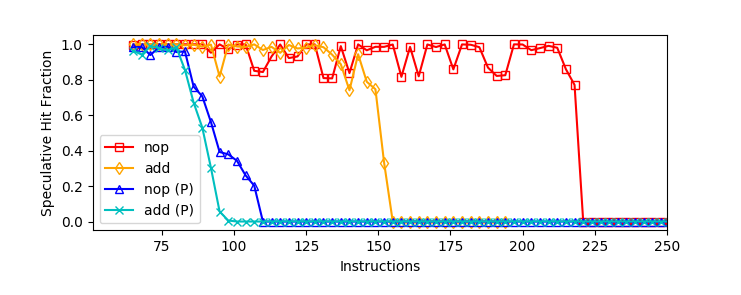
\includegraphics[width=1.05\linewidth]{figures/Speculative_measurements_parity.png}
        \caption{\textbf{Hyperthreading}\,---\,% The trigger program influences
        the payload program via the indirect branch predictor when running on
        the same logical CPU core. Hyperthreads also share an indirect branch
        predictor despite running on different logical cores. We measured the
        impact of same logical core (warm colors) vs parity hyperthreads (cool
        colors, denoted by (P)) on the size of the speculative execution window.
        As hyperthreads run concurrently, they do not need to wait for an OS
        context switch between processes, but the two processes directly contend
        for ROB entries. As a result, we find that hyperthreads generally have a
        smaller speculative execution window.}
    \label{fig:spec-capacity-parity}
\end{figure}
}


\newcommand{\FigSpecMeasure}{
\begin{figure*}[t]
     \centering
        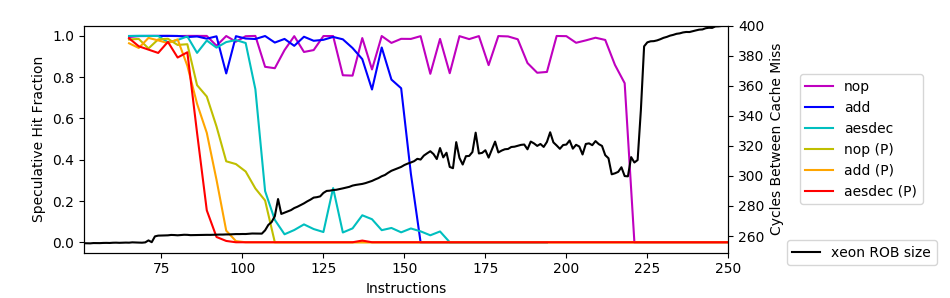
\includegraphics[width=0.9\textwidth]{figures/Speculative_measurements.png}
    \caption{The speculative primitive allows for a limited number of instructions
        to be completed speculatively, dependent on multiple factors. Trigger and 
        payload processes must share CPU resources as they must be performed on 
        the same hyperthread or associated parity hyperthreads. Processes on
        the parity hyperthreads (warm colors) denoted by (P) accomplish a 
        significantly lower number of instructions as compared with processes 
        on the same hyperthread (cool colors).}
    \label{fig:spec-capacity}
\end{figure*}
}


\newcommand{\FigCacheMiss}{
\begin{figure}[t]
    \centering
    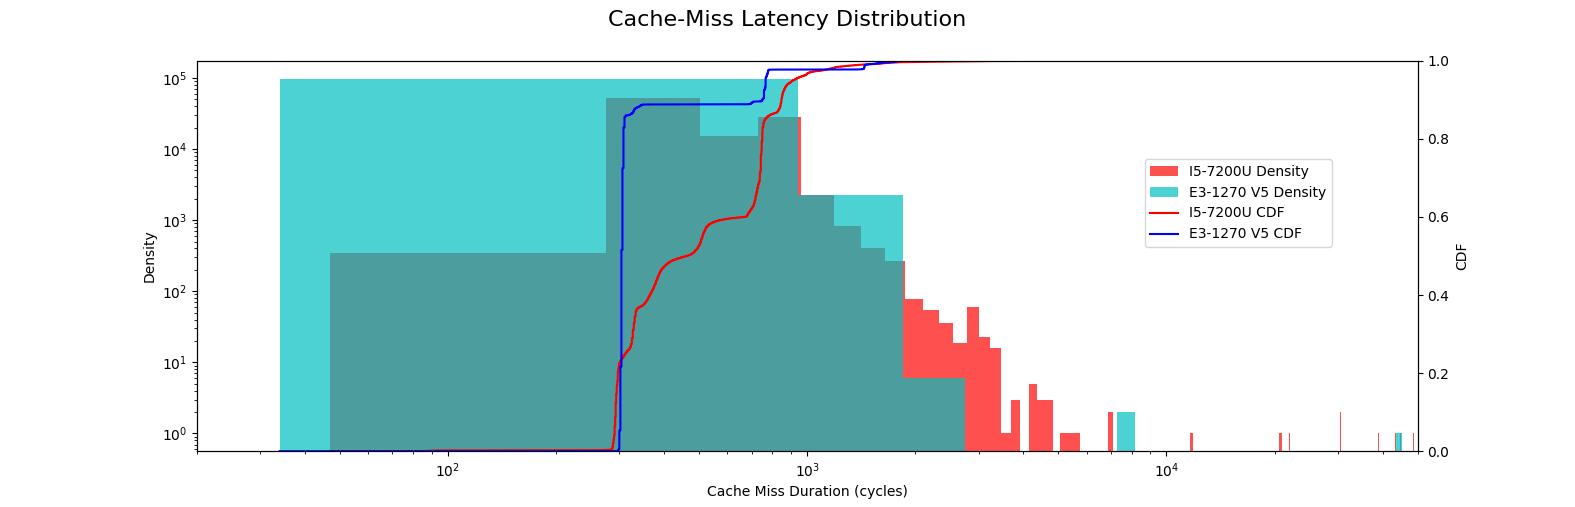
\includegraphics[width=0.5\textwidth]{figures/cache_miss_dist}
    \caption{\textbf{Cache latency}\,---\,%
        Cumulative distribution function of the cache hit and miss latency
        for an Intel Xeon-1270 and AMD Epyc 7251. If a cache miss is used
        to force CPU speculation, the CPU must wait at least 300-800 cycles
        before the speculated branch can be resolved. However, we find the CPU
        can execute far fewer instructions speculatively, suggesting another
        limit is at play.}
    \label{fig:cache-miss}
\end{figure}
}


\newcommand{\FigGeneralModel}{
\begin{figure}[t]
    \centering
        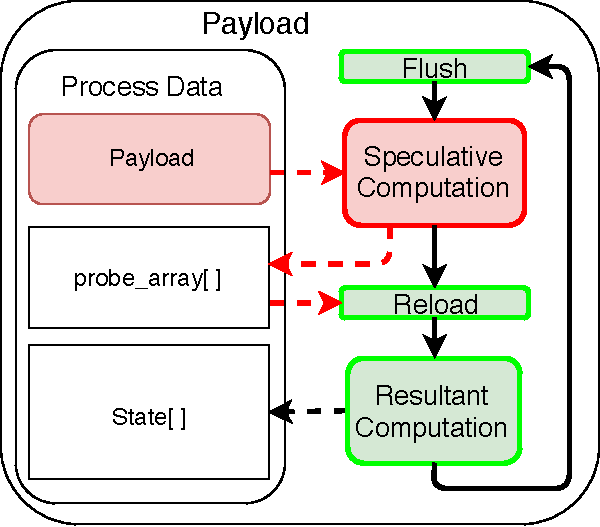
\includegraphics[width=0.4\textwidth]{figures/general_model.pdf}
        \caption{\textbf{ExSpectre model}\,---\,%
        General model of speculative computation within the payload 
        process when triggered. The \textit{Speculative Gadget} has read-only
        access to all memory within the process, but can return updates/results via a
        cache side channel (via access to the \texttt{probe\_array}).
        The process can subsequently make
        \textit{Resultant Computations} based on the value returned from
        the cache side channel to update the state of the \textit{Real World} process.}
    \label{fig:general_model}
\end{figure}
}


\newcommand{\FigSpecBandwidth}{
\begin{figure}[t]
    \centering  
        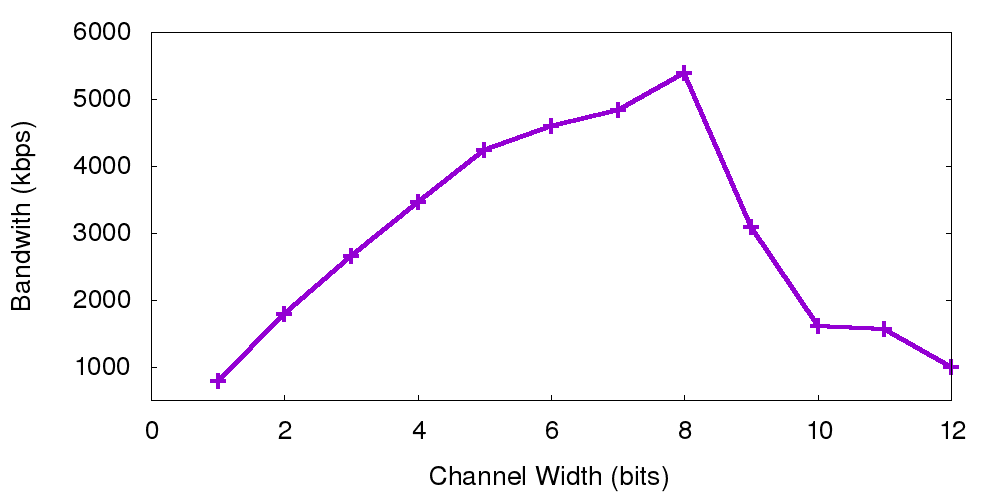
\includegraphics[width=0.5\textwidth]{figures/Speculative_bandwidth}
        \caption{\textbf{Speculative Bandwidth}\,---\,%
        Using our speculative primitive, 1KB of data
        can be decrypted and exfiltrated at a speed of 5.38~Kbps from
        the speculative world with 20 redundant iterations per round (to ensure
        correctness). Increased channel width exfiltrates more data per round,
        but takes longer to measure the cache side channel. Optimal throughput is
        achieved with an 8-bit channel.}
    \label{fig:spec_bandwidth}
\end{figure}
}

\newcommand{\FigSpasmModel}{
\begin{figure}[b]
    \centering
        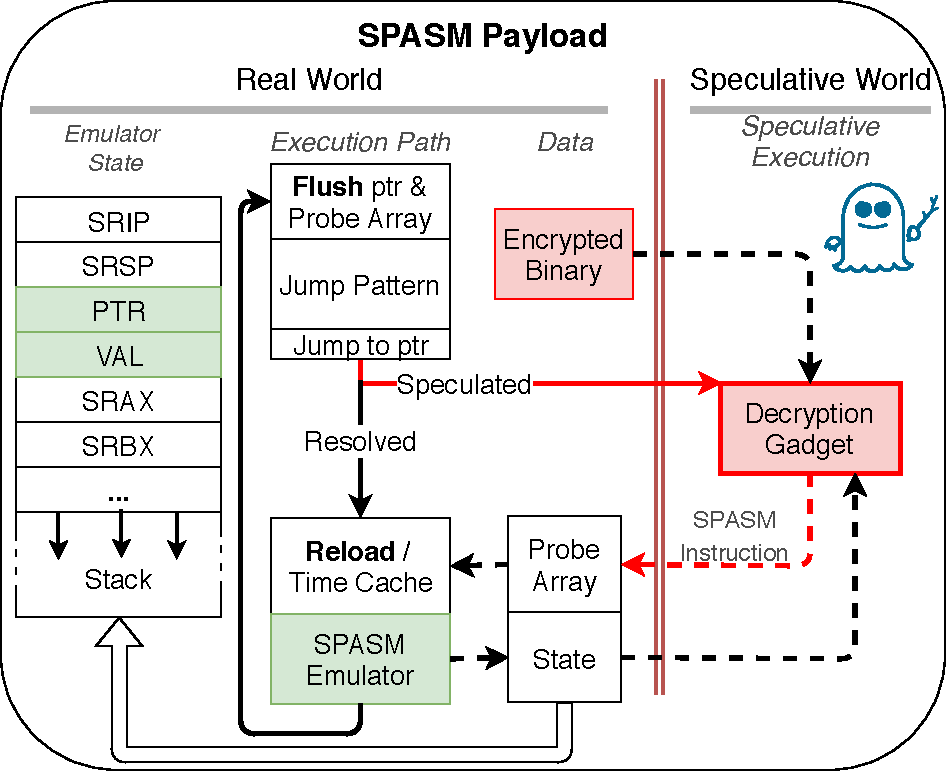
\includegraphics[width=0.46\textwidth]{figures/spasm_model.pdf}
        \caption{\textbf{SPASM model}\,---\,%
        Our SPASM emulator speculatively decrypts instructions, and emulates
        them in the real world. The \textit{Speculative Computation} decrypts
        the encrypted SPASM binary, returning the result through the side channel
        to allow the \textit{Resultant Computation} to update the emulated state
        (or make system calls) on behalf of the speculative world.}
    \label{fig:spasm_model}
\end{figure}
}

\newcommand{\FigTuringSuccess}{
\begin{figure}[t]
    \centering
        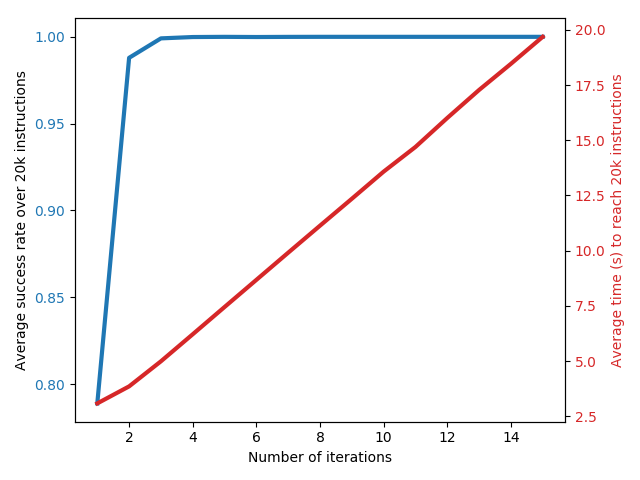
\includegraphics[width=0.46\textwidth]{figures/SuccessAndTime}

    \caption{The number of steps and error rate of a the 5-state Busy
            Beaver configuration were measured as a function of how many
            (redundant) iterations into the speculative world were performed. As
            expected, the amount of time to complete a million steps is a
            linear function of how many indirect calls into the speculative
            world we take. Additionally we see that it only requires using 10
            speculative calls per step to achieve a very low number of
            errors in reaching a million instructions, making 10-20 steps
            an attractive choice for most applications.}

    \label{fig:turing_success}
\end{figure}
}

\newcommand{\processorTable}{
\begin{table}
    \centering
    % \resizebox{\linewidth}{!}{\begin{tabularx}{\linewidth}{X X X| Y Y Y}
    \begin{tabularx}{\linewidth}{X b b| Y Y Y}
        \ \newline
        \ \newline
        Processor & \ \newline
        Year\newline
        released & \ \newline
        Micro\newline
        arch & \ \newline
        Nested\newline 
        Spec? & Num\newline
        indirect jumps* & Max $\mu$~ops\newline
        (nop)\\
        \hline
        Intel Xeon CPU E3-1270 v6 & 2017 & Skylake & \checkmark & 28 & 220\\
        Intel Core i5-7200U       & 2016 & Skylake & \checkmark & 26 & 220\\
        Intel Xeon CPU E3-1276 v3 & 2014 & Haswell &            & 26 & 178\\
        AMD EPYC 7251             & 2017 & Ryzen   &            & 4  & 178\\
        \\
    \end{tabularx}%}
    \caption{\textbf{Processor features}--- We analyzed the capability of
    \speculake on one AMD and three Intel processors. Both Skylake processors
    were capable of nested speculation (Section~\ref{sssec:nested-spec}) though
    the older Haswell processor and the AMD processor were not. We found that
    the Intel Xeon CPU E3-1270 v6 required 28 identical indirect jumps in the
    trigger and payload programs to reliably enter the speculative world at the
    desired speculative entry point ($> 95\%$) while the Intel Core i5-7200U
    and Intel Xeon CPU E3-1276 v3 only required 26 jumps. The AMD EPYC 7251
    processor maintained a 85\% speculative hit rate with as low as 4 and as
    high as 32 training jumps.}
    \label{table:processors}
\end{table}
}
